% This is "sig-alternate.tex" V1.9 April 2009
% This file should be compiled with V2.4 of "sig-alternate.cls" April 2009
%
% This example file demonstrates the use of the 'sig-alternate.cls'
% V2.4 LaTeX2e document class file. It is for those submitting
% articles to ACM Conference Proceedings WHO DO NOT WISH TO
% STRICTLY ADHERE TO THE SIGS (PUBS-BOARD-ENDORSED) STYLE.
% The 'sig-alternate.cls' file will produce a similar-looking,
% albeit, 'tighter' paper resulting in, invariably, fewer pages.
%
% ----------------------------------------------------------------------------------------------------------------
% This .tex file (and associated .cls V2.4) produces:
%       1) The Permission Statement
%       2) The Conference (location) Info information
%       3) The Copyright Line with ACM data
%       4) NO page numbers
%
% as against the acm_proc_article-sp.cls file which
% DOES NOT produce 1) thru' 3) above.
%
% Using 'sig-alternate.cls' you have control, however, from within
% the source .tex file, over both the CopyrightYear
% (defaulted to 200X) and the ACM Copyright Data
% (defaulted to X-XXXXX-XX-X/XX/XX).
% e.g.
% \CopyrightYear{2007} will cause 2007 to appear in the copyright line.
% \crdata{0-12345-67-8/90/12} will cause 0-12345-67-8/90/12 to appear in the copyright line.
%
% ---------------------------------------------------------------------------------------------------------------
% This .tex source is an example which *does* use
% the .bib file (from which the .bbl file % is produced).
% REMEMBER HOWEVER: After having produced the .bbl file,
% and prior to final submission, you *NEED* to 'insert'
% your .bbl file into your source .tex file so as to provide
% ONE 'self-contained' source file.
%
% ================= IF YOU HAVE QUESTIONS =======================
% Questions regarding the SIGS styles, SIGS policies and
% procedures, Conferences etc. should be sent to
% Adrienne Griscti (griscti@acm.org)
%
% Technical questions _only_ to
% Gerald Murray (murray@hq.acm.org)
% ===============================================================
%
% For tracking purposes - this is V1.9 - April 2009

\documentclass{sig-alternate}
  \pdfpagewidth=8.5truein
  \pdfpageheight=11truein
  

\usepackage{algorithm}
\usepackage[noend]{algpseudocode}
\usepackage{graphicx}

\begin{document}
%
% --- Author Metadata here ---
\conferenceinfo{SAC'15}{January 1 - April 31, 2016, Boulder, CO.}
\CopyrightYear{2016} % Allows default copyright year (2002) to be over-ridden - IF NEED BE.
\crdata{978-1-4503-3196-01/2016/01}  % Allows default copyright data (X-XXXXX-XX-X/XX/XX) to be over-ridden.
% --- End of Author Metadata ---

\title{Backtracking Sudoku Solver}
%
% You need the command \numberofauthors to handle the 'placement
% and alignment' of the authors beneath the title.
%
% For aesthetic reasons, we recommend 'three authors at a time'
% i.e. three 'name/affiliation blocks' be placed beneath the title.
%
% NOTE: You are NOT restricted in how many 'rows' of
% "name/affiliations" may appear. We just ask that you restrict
% the number of 'columns' to three.
%
% Because of the available 'opening page real-estate'
% we ask you to refrain from putting more than six authors
% (two rows with three columns) beneath the article title.
% More than six makes the first-page appear very cluttered indeed.
%
% Use the \alignauthor commands to handle the names
% and affiliations for an 'aesthetic maximum' of six authors.
% Add names, affiliations, addresses for
% the seventh etc. author(s) as the argument for the
% \additionalauthors command.
% These 'additional authors' will be output/set for you
% without further effort on your part as the last section in
% the body of your article BEFORE References or any Appendices.

\numberofauthors{1} %  in this sample file, there are a *total*
% of EIGHT authors. SIX appear on the 'first-page' (for formatting
% reasons) and the remaining two appear in the \additionalauthors section.
%
\author{
% You can go ahead and credit any number of authors here,
% e.g. one 'row of three' or two rows (consisting of one row of three
% and a second row of one, two or three).
%
% The command \alignauthor (no curly braces needed) should
% precede each author name, affiliation/snail-mail address and
% e-mail address. Additionally, tag each line of
% affiliation/address with \affaddr, and tag the
% e-mail address with \email.
%
% 1st. author
\alignauthor
Nicolas C. Broeking\\
       \affaddr{University of Colorado at Boulder}\\
       \affaddr{Advanced Algorithms}\\
       \affaddr{CSCI 5454}\\
       \email{nibr3402@colorado.edu}
% 2nd. author
}


\maketitle
\begin{abstract}
In this project, I successfully implemented a Sudoku Backtracking Solver written in python. Using this algorithm, I prove that the runtime in the worst case is $O(n^{2*^{n^4} + 2})$ but by introducing a variable m, where m is the number of unfilled squares, I am able to show a tighter runtime of $O(n^{2*m})$. Then I am able to show the space complexity of the algorithm to be $O(n^4)$. Finally, I analyze the types of inputs into the algorithm and show the worst, average, and best case inputs for the algorithm. 
\end{abstract}

% A category with the (minimum) three required fields
\category{H.4}{Algorithms}{Sudoku}{Backtracking}{Search}
%A category including the fourth, optional field follows...

\terms{Search}

\keywords{Sudoku, Search, Backtracking Search}

\section{Introduction}
Sudoku is a popular game played by puzzle enthusiasts all over the world where the player takes 
a grid of size $n^2 x n^2$ with some hints filled in and then tries to fill in the rest of the grid. \cite{YasSS} The most common form of sudoku is the $n=3$ form which is a 9x9 grid. Which looks like: 

\begin{center}
  \begin{tabular}{ | c | c | c | c | c | c | c | c | c |}
    \hline
     & & & & 1 & 5 & & & 3 \\ \hline
	 & & 8 & 3 & & 2 & & & 4 \\ \hline
	 & & & & 8 & 6 & & & \\ \hline
	 & 7 & & & & & & & \\ \hline
	 & & & 1 & & & 2 & 8 & 7\\ \hline
	 & & 5 & & 6 & & 9 & & \\ \hline
     8 & & 9 & & & & & & \\ \hline
	 & 1 & 2 & & & & & 9 & 8\\ \hline
	 4 & 6 & 3 & & & & & & \\ \hline
  \end{tabular}
\end{center}

The sudoku has a solution if the following three rules are true. 

\begin{itemize}
\item{All blocks are filled in with an integer x where $0 < x \le n^2$}
\item{There are no duplicate numbers in a given row}
\item{There are no duplicate numbers in a given col}
\item{There are no duplicate numbers in any given sub square}
\end{itemize}

Following the rules of the game, we are able to solve the above example as: 

\begin{center}
  \begin{tabular}{ | c | c | c | c | c | c | c | c | c |}
    \hline
     6 & 2 & 4 & 9 & 1 & 5 & 8 & 7 & 3 \\ \hline
	 1 & 9 & 8 & 3 & 7 & 2 & 6 & 5 & 4 \\ \hline
	 5 & 3 & 7 & 4 & 8 & 6 & 1 & 3 & 9\\ \hline
	 2 & 7 & 1 & 8 & 4 & 9 & 3 & 6 & 5\\ \hline
	 9 & 4 & 6 & 1 & 5 & 3 & 2 & 8 & 7\\ \hline
	 3 & 8 & 5 & 2 & 6 & 7 & 9 & 4 & 1\\ \hline
     8 & 5 & 9 & 7 & 2 & 1 & 4 & 3 & 6\\ \hline
	 7 & 1 & 2 & 6 & 3 & 4 & 5 & 9 & 8\\ \hline
	 4 & 6 & 3 & 5 & 9 & 8 & 7 & 1 & 2\\ \hline
  \end{tabular}
\end{center}

In this paper I explore how to apply a backtracking algorithm to the sudoku problem to solve Sudoku puzzles of various sizes. To do this we search the tree space trying different values in each square and then searching sub trees. 

Next I analyze the the running time of the algorithm to determine a worst case runtime of $O(n^{2*^{n^4} + 2})$. This runtime is established based off of the search space size plus the work that needs to be done at every level. Unfortunately, the worst case bound for this does not take into account hints. 

Then we introduce a variable, m where m is the number unfilled boxes. We are able to redefine the runtime to be $O(n^{2*m})$. This provides a tighter bound on the runtime. 

Next we investigate the memory space to prove that the space complexity is $O(n^4)$. All operations in the algorithm are performed in place and thus we only need memory to keep track of the game state. 

Finally, we look at the best, average and worst case inputs for the algorithm. We can show that the worst case input for the algorithm is a game state that requires the most backtracking. The average case is when there are enough hints to have only one solution. The best case is when the hints allow the backtracking algorithm to guess the correct value at each box on the first try. 

\section{Problem}
The Sudoku Solving Problem, in the form of $n^2 x n^2$, is a NP-Complete problem. \cite{YATO}. It has been shown to easily be converted to another problem known as the Latin Square. The Latin Square problem can essentially is the sub problem for each of Sudoku Sub Squares. In this paper we are not diving into the showing NP-Completeness for Sudoku but we can take advantage of this fact to develop a backtracking algorithm to solve the problem. The algorithm essentially boils down to a graph coloring where each block is a node and a block can be colored any number x where $0 < x \le n^2$. The rules for the graph coloring remain the same as the rules specified above. 
\cite{YATO}

%---------------------------------------------------
\section{Algorithm}
The Sudoku Backtracking algorithm conceptually is a very simple algorithm. It takes a matrix G where G is partially filled in with values. We call these values hints. Then it recursively looks through the graph. Essentially performing a depth first search. Each level in the graph is a box and it branches with different values. The algorithm tries a value in a box A. If none of the rules of Sudoku are violated it then recurses down to the next box B and tries a value. If at anytime a value breaks one of the rules of the tree it immediately returns none and will then try another value in the box. 

\subsection{Example}

Assume we have a Matrix M that looks like:

\begin{center}
  \begin{tabular}{ | c | c | c | c | c | c | c | c | c |}
    \hline
      & 2 & 4 & 9 &  & 5 & 8 & 7 & 3 \\ \hline
	  & 9 & 8 & 3 & 7 & 2 & 6 & 5 & 4 \\ \hline
	 5 & 3 & 7 & 4 & 8 & 6 & 1 & 3 & 9\\ \hline
	 2 & 7 & 1 & 8 & 4 & 9 & 3 & 6 & 5\\ \hline
	 9 & 4 & 6 & 1 & 5 & 3 & 2 & 8 & 7\\ \hline
	 3 & 8 & 5 & 2 & 6 & 7 & 9 & 4 & 1\\ \hline
     8 & 5 & 9 & 7 & 2 & 1 & 4 & 3 & 6\\ \hline
	 7 & 1 & 2 & 6 & 3 & 4 & 5 & 9 & 8\\ \hline
	 4 & 6 & 3 & 5 & 9 & 8 & 7 & 1 & 2\\ \hline
  \end{tabular}
\end{center}

The algorithm first starts at the first square and will try a 1. 

\begin{center}
  \begin{tabular}{ | c | c | c | c | c | c | c | c | c |}
    \hline
      \textbf{1} & 2 & 4 & 9 &  & 5 & 8 & 7 & 3 \\ \hline
	  & 9 & 8 & 3 & 7 & 2 & 6 & 5 & 4 \\ \hline
	 5 & 3 & 7 & 4 & 8 & 6 & 1 & 3 & 9\\ \hline
	 2 & 7 & 1 & 8 & 4 & 9 & 3 & 6 & 5\\ \hline
	 9 & 4 & 6 & 1 & 5 & 3 & 2 & 8 & 7\\ \hline
	 3 & 8 & 5 & 2 & 6 & 7 & 9 & 4 & 1\\ \hline
     8 & 5 & 9 & 7 & 2 & 1 & 4 & 3 & 6\\ \hline
	 7 & 1 & 2 & 6 & 3 & 4 & 5 & 9 & 8\\ \hline
	 4 & 6 & 3 & 5 & 9 & 8 & 7 & 1 & 2\\ \hline
  \end{tabular}
\end{center}

None of the rules of sudoku have been violated so it then recurses to the next empty square. It will try a 1 in the next square. 

\begin{center}
  \begin{tabular}{ | c | c | c | c | c | c | c | c | c |}
    \hline
      \textbf{1} & 2 & 4 & 9 &  \textbf{1} & 5 & 8 & 7 & 3 \\ \hline
	  & 9 & 8 & 3 & 7 & 2 & 6 & 5 & 4 \\ \hline
	 5 & 3 & 7 & 4 & 8 & 6 & 1 & 3 & 9\\ \hline
	 2 & 7 & 1 & 8 & 4 & 9 & 3 & 6 & 5\\ \hline
	 9 & 4 & 6 & 1 & 5 & 3 & 2 & 8 & 7\\ \hline
	 3 & 8 & 5 & 2 & 6 & 7 & 9 & 4 & 1\\ \hline
     8 & 5 & 9 & 7 & 2 & 1 & 4 & 3 & 6\\ \hline
	 7 & 1 & 2 & 6 & 3 & 4 & 5 & 9 & 8\\ \hline
	 4 & 6 & 3 & 5 & 9 & 8 & 7 & 1 & 2\\ \hline
  \end{tabular}
\end{center}

Obviously there can't be two 1's in a row so it keeps checking values 1 - 9. All of them violate the rules so the algorithm backtracks back to the first square. The first square keeps trying values until it finds one that doesn't brake any rules. It lands on a 6. 

\begin{center}
  \begin{tabular}{ | c | c | c | c | c | c | c | c | c |}
    \hline
      \textbf{6} & 2 & 4 & 9 &  & 5 & 8 & 7 & 3 \\ \hline
	  & 9 & 8 & 3 & 7 & 2 & 6 & 5 & 4 \\ \hline
	 5 & 3 & 7 & 4 & 8 & 6 & 1 & 3 & 9\\ \hline
	 2 & 7 & 1 & 8 & 4 & 9 & 3 & 6 & 5\\ \hline
	 9 & 4 & 6 & 1 & 5 & 3 & 2 & 8 & 7\\ \hline
	 3 & 8 & 5 & 2 & 6 & 7 & 9 & 4 & 1\\ \hline
     8 & 5 & 9 & 7 & 2 & 1 & 4 & 3 & 6\\ \hline
	 7 & 1 & 2 & 6 & 3 & 4 & 5 & 9 & 8\\ \hline
	 4 & 6 & 3 & 5 & 9 & 8 & 7 & 1 & 2\\ \hline
  \end{tabular}
\end{center}

Once it finds 6, there are no conflicts so it recurses back down and tries the 1 in the next open box.

\begin{center}
  \begin{tabular}{ | c | c | c | c | c | c | c | c | c |}
    \hline
      \textbf{6} & 2 & 4 & 9 & \textbf{1} & 5 & 8 & 7 & 3 \\ \hline
	  & 9 & 8 & 3 & 7 & 2 & 6 & 5 & 4 \\ \hline
	 5 & 3 & 7 & 4 & 8 & 6 & 1 & 3 & 9\\ \hline
	 2 & 7 & 1 & 8 & 4 & 9 & 3 & 6 & 5\\ \hline
	 9 & 4 & 6 & 1 & 5 & 3 & 2 & 8 & 7\\ \hline
	 3 & 8 & 5 & 2 & 6 & 7 & 9 & 4 & 1\\ \hline
     8 & 5 & 9 & 7 & 2 & 1 & 4 & 3 & 6\\ \hline
	 7 & 1 & 2 & 6 & 3 & 4 & 5 & 9 & 8\\ \hline
	 4 & 6 & 3 & 5 & 9 & 8 & 7 & 1 & 2\\ \hline
  \end{tabular}
\end{center}

Finally, it recurses to the last empty box and tries a 1.

\begin{center}
  \begin{tabular}{ | c | c | c | c | c | c | c | c | c |}
    \hline
      \textbf{6} & 2 & 4 & 9 & \textbf{1} & 5 & 8 & 7 & 3 \\ \hline
	 \textbf{1} & 9 & 8 & 3 & 7 & 2 & 6 & 5 & 4 \\ \hline
	 5 & 3 & 7 & 4 & 8 & 6 & 1 & 3 & 9\\ \hline
	 2 & 7 & 1 & 8 & 4 & 9 & 3 & 6 & 5\\ \hline
	 9 & 4 & 6 & 1 & 5 & 3 & 2 & 8 & 7\\ \hline
	 3 & 8 & 5 & 2 & 6 & 7 & 9 & 4 & 1\\ \hline
     8 & 5 & 9 & 7 & 2 & 1 & 4 & 3 & 6\\ \hline
	 7 & 1 & 2 & 6 & 3 & 4 & 5 & 9 & 8\\ \hline
	 4 & 6 & 3 & 5 & 9 & 8 & 7 & 1 & 2\\ \hline
  \end{tabular}
\end{center}

There are no conflicts on this last matrix and all values are filled in and thus we have a valid solution. 

\subsection{Pseudocode}

So now that we have defined the algorithms behavior lets define the algorithms pseudocode.

\begin{algorithm}[H]
\caption{Sudoku Backtracking}\label{solve}
\begin{algorithmic}[1]
\Procedure{solve}{G, box}

\If{reject (G)}
\State return None
\EndIf

\If{accept(G)}
\State return G
\EndIf

\If $box \ge n^4$
\State return None
\EndIf

\State x, y = getIndices(box, size)

\If{ !self.isempty(G[x][y])}
\State return solve(G, box+1)
\EndIf

\For{ index $i < n^2$}
\State $G'$[x][y] = i
\State solution = solve($G'$, box + 1)
\If{result !=None}
\State return Result
\EndIf
\EndFor
\State G[x][y] = 0
\State Return None
\EndProcedure
\end{algorithmic}
\end{algorithm}

\cite{GeeksforGeeks}
\cite{Backtracking}

The algorithm above performs the backtracking and will correctly solve all valid sudoku puzzles. For puzzles that do not have valid solutions the algorithm returns None. However it depends on the following 4 subroutines. 

Now lets look at each of the subroutines one by one. 

%Reject sub routine
\subsubsection{Reject}
The reject subroutine takes a Graph G and then checks to see if there is there is a possible solution given G. For example if the G passed to it has two threes in a single column then reject will return True saying that there is no solution because you can't have more than one of each number in any given column. 

This subroutine is extremely powerful because it allows us to prune the tree for huge sub-trees at a time. As we will show later the game state for sudoku is massive so any time that we are able to prune we see massive speed ups in  Given any two squares of the same value there are potentially $9^(n^4 - 2)$ sub states that can we don't need to search because we know they can't be valid. 


\begin{algorithm}[H]
\caption{Reject}\label{reject}
\begin{algorithmic}[1]
\Procedure{reject}{G}
\For{ index $i < n^2$}
\State $x = set()$
\For{ index $j < n^2$}
\If{matrix[i][j] > 0}
\If{matrix[i][j] in x}
\State return True
\EndIf
\State x.add(matrix[i][j])
\EndIf
\EndFor
\EndFor
\For{ index $j < n^2$}
\State $y = set()$
\For{ index $i < n^2$}
\If{ matrix[i][j] > 0}
\If{ matrix[i][j] in y}
\State return True
\EndIf
\State y.add(matrix[i][j])
\EndIf
\EndFor
\EndFor
\For{ index $offsetx < n^2$}
\For{ index $offsety < n^2$}
\State valid = set()
\For{ index $i < n^2$}
\For{ index $j < n^2$}
\State indexX = offsetx*n + i
\State indexY = offsetY*n + j
\If{ $matrix[indexX][indexY] > 0$}
\If{ matrix[indexx][indexy] in valid }
\State return True
\EndIf
\State valid.add(matrix[indexX][indexY]
\EndIf
\EndFor
\EndFor
\EndFor
\EndFor
\State return False
\EndProcedure
\end{algorithmic}
\end{algorithm}

\cite{Backtracking}

%Accept sub routine
\subsubsection{Accept}
The accept subroutine looks very similar to reject but instead of determining if given G is there a set of open values that leads to a solvable solution. What does this mean? Well for accept to return true all of the Sudoku's rules must be satisfied.

\begin{algorithm}[H]
\caption{Accept}\label{accept}
\begin{algorithmic}[1]
\Procedure{accept}{G}

\For{ index $i < n^2$}
\State $x = set()$
\For{ index $j < n^2$}
\If{ matrix[i][j] > 0}
\If{ matrix[i][j] in x}
\State return False
\EndIf
\State x.add(matrix[i][j])
\Else
\State return False
\EndIf
\EndFor
\EndFor

\For{ index $j < n^2$}
\State $y = set()$
\For{ index $i < n^2$}
\If {matrix[i][j] > 0}
\If {matrix[i][j] in y}
\State return False
\EndIf
\State y.add(matrix[i][j])
\Else
\State return False
\EndIf
\EndFor
\EndFor

\For{ index $offsetx < n^2$}
\For{ index $offsety < n^2$}
\State valid = set()
\For{ index $i < n^2$}
\For{ index $j < n^2$}
\State indexX = offsetx*n + i
\State indexY = offsetY*n + j

\If {$matrix[indexX][indexY] > 0$}
\If {matrix[indexx][indexy] in valid }
\State return False
\EndIf
\State valid.add(matrix[indexX][indexY]
\Else
\State return False
\EndIf
    
\EndFor
\EndFor
\EndFor
\EndFor
\State return True
\EndProcedure
\end{algorithmic}
\end{algorithm}
\cite{Backtracking}

\subsubsection{getIndices}
Get Indices is a small subroutine that I am only including for completeness of the algorithm. GetIndices takes a recursion depth of the tree, x where x represents the current box. X can be any integer as long as $ 0 \le x < n^4$. Get Indices then returns a tuple that represents the corresponding x and y indices of the box in the matrix representation. This allows us to do a conversion between recursion depth and indices into the matrix . Referencing the recursion from the box number then guarantees that we have a max recursion depth of $n^4$ where the box matches the recursion depth. 

GetIndices takes a integer i and n and returns a tuple of the x and y indices that correspond to that frame.

\begin{algorithm}[H]
\caption{getIndices}\label{getIndecies}
\begin{algorithmic}[1]
\Procedure{getIndces}{index}

\State return ( $index / n^2$, $index \% n^2$)

\EndProcedure
\end{algorithmic}
\end{algorithm}


\subsubsection{Isempty}

The is empty subroutine is the last subroutine and just like GetIndices it is very trivial. It is used to check to see if any particular value in the matrix has been filled. My implementation chooses to use 0 to represent an empty field. If a field then has a 0 we know it to be empty and if it has a value x where $0 < x \le n^2$ then it is filled in with value x. 

\begin{algorithm}[H]
\caption{isempty}\label{isempty}
\begin{algorithmic}[1]
\Procedure{isempty}{val}
\State return $True ? val <= 0 : False$
\EndProcedure
\end{algorithmic}
\end{algorithm}


%---------------------------------------------------
\section{Correctness}

Now that we talked about exactly what the algorithm is doing we can dive in to how we can be sure the algorithm is doing what we expect. We can prove its correctness by first looking at the solver as a whole and proving the main algorithm correct and then proving its subroutines correct. 

\subsection{Sudoku Backtracking Solver}
We can be sure the Sudoku Backtracking Algorithm is correct if and only if it returns a valid solution if one exists or None if a valid solution does not exist. A Sudoku puzzle is said to have a solution if each of the following rules are satisfied. 
\begin{itemize}
\item{$\forall val \in Grid \quad 0 < val < n^2$} 
\item{$\forall row \in Rows$ row has $n^2$ unique non zero values}
\item{$\forall col \in Cols$ col has $n^2$ unique non zero values}
\item{$\forall square \in Squares$ square has $n^2$ unique non zero values}
\item{$\forall val \in Original Grid$ val does not change}
\end{itemize}

Using this information I am able to construct the following proof. 

\textbf{Claim: Sudoku Backtracking solver returns a valid solution if one exists or None if a valid solution does not exist}
\begin{proof}
The Sudoku solver is a backtracking recursive algorithm. To prove its correctness we first look at its base cases and prove with induction. 

We have three base cases: Reject, Accept and out of values. Given a matrix G we terminate if either we accept the matrix G, reject the Matrix G, or have exhausted all possible options. These three options provide an exhaustible and complete set of possible results showing that the Algorithm will always terminate at one event. 

Given a graph G we first check if it is possible to have a solution. If it isn't we immediately return None proving we can detect invalid Sudoku squares. Given the same graph G once we check if it is possible to have a solution we then check if G is a valid solution. If it is we return it immediately proving we can detect a valid solution. If either one of these are true the next step is to guess a value and then recurse as the induction step.

The induction step is to  guess a value and then recurse. To do this we fill in a value for box n and then recurse on the subgraph. As I just showed, this recursion will always terminate as thus have shown that the algorithm will recursively select values until we find a valid solution. 

The only other thing we havn't shown is how to handle the hints that are fed into the original question. By checking if a value already exists and then just recursing one layer down we ensure we don't change any values given to the algorithm as hints while returning whatever the recursion allows. 

Ensuring that for any given graph G and recursion depth n we can find a solution then we know that for any G and recursion depth we are able to find a solution proving that Sudoku Backtracking solver returns a valid solution if one exists or None if a valid solution does not exist.
\end{proof}

\subsection{Reject}
If we have a $n^2$ x $n^2$ matrix. Then we have 3 sets: Rows, Cols, and Squares. Rows is the set of $n^2$ rows. Cols is the set of $n^2$ cols and squares contains $n^2$ non overlapping squares of size n x n. To show correctness the algorithm needs to reject the matrix if one of three conditions is true. 
\begin{itemize}
\item{$\forall row \in Rows$ row has $n^2$ unique non zero values}
\item{$\forall col \in Cols$ col has $n^2$ unique non zero values}
\item{$\forall square \in Squares$ square has $n^2$ unique non zero values}
\end{itemize}

\textbf{Reject will return true if no such possible solution exists or false if a solution can still be found. }
\begin{proof}

Assume that we have a matrix that has a duplicate in a random given row. We know that this matrix is invalid because of rule one. The first for loop in the reject subroutine then will check each element in each row. Adding it to a set for each row. If that set has a conflict we guarantee that there is a duplicate and thus reject will correctly return true. Each individual value only gets added to the set if a non 0 value gets added to the set therefore we are only checking values in the matrix that the algorithm has found proving that any violation of rule 1 will get caught. \\

Now assume that we have a matrix that has a duplicate value in a random col.
We know that the matrix is invalid because of rule two. The second loop in the subroutine iterates all the columns and for each column adds each columns non 0 values to the set. When there is a conflict in the set because of the duplicate value then we guarantee to return true and will reject the invalid matrix. 

Next assume we have a matrix that has a duplicate value in one of its sub-squares. Then we know the matrix is invalid because of rule three. The third and final loop in the subroutine iterates the squares and for each square adds all elements into a set. If there is a conflict then we guarantee that there was a duplicate in the square and return true. 

Finally, we can assume we have a matrix that has does not violate any of the rules then the reject subroutine does not flag anything. If there are no duplicates in each individual row then there will be now conflict adding the values to the set so nothing will get flagged. If there are no duplicates in the columns then there wont be a conflict with the column sets and therefore wont be flagged. Finally if there are no duplicates in the squares then there wont be a conflict adding things to the squares set and therefore nothing will get flagged. Leaving the last instruction to return false which does not reject the matrix. 

Thus proving that the reject function will return true if any of Sudoku rules are violated and false if not. 
\end{proof}

\subsection{Accept}
Accept is extremely similar to reject but instead of checking if there is a chance of finding a correct solution we must ensure that the matrix G is a valid solution. Given this information we know that we can accept a grid the following four rules are true. 

\begin{itemize}
\item{$\forall val \in Grid \quad 0 < val < n^2$} 
\item{$\forall row \in Rows$ row has $n^2$ unique non zero values}
\item{$\forall col \in Cols$ col has $n^2$ unique non zero values}
\item{$\forall square \in Squares$ square has $n^2$ unique non zero values}
\end{itemize}

\textbf{Accept will return true if G is a valid solution else will return false}
\begin{proof}
Assume we have valid grid then searching through each row in the first set of loops will ensure that there are no duplicates and that each value has been filled in. If one of these requirements was not bet the algorithm will short circuit ensuring that the rule 1 and 2 are met. 

After ensuring the rows are correct we then need to ensure that all columns have a unique value. The second set of loops ensures that every value in a given row is unique and will short circuit false if rule 3 is not met. We can ensure this because the loops are creating a set for each row and adding values to it. If there is ever a conflict then we know there can't be a valid solution, returning false.

Finally, we need to ensure that every square has a unique value. The third and final set of loops iterate all values inside each non overlapping square ensuring that this rule is met. 

In all steps if we see any non 0 value we short circuit. 

Ensuring that each of these 4 rules is satisfied the last step is to return true proving that Accept will return true if G is a valid solution else it will return false. 
\end{proof}

\subsection{Get Indices}
The get indices function is designed to convert any integer $0 \le i \le n^4$ to the corresponding tuple that represents indices into the Sudoku grid.

\textbf{Get Indices returns a tuple (x,y) where x is the row index and y is the column index}
\begin{proof}
If we have an matrix M where M is size $n^2 x n^2$ then index i is equal to the $i/n^2$ row and the $i\%n^2$ column. Formally we can write this as Given an integer i where $0 \le i \le n^4$ getIndices(i) will return ($i/n^2$, $i\%n^2$). The subroutine returns this mathematical expression exactly proving that Get Indeces returns a tuple (x,y) where x is the row index and y is the column index.
\end{proof}

\subsection{Is Empty}
\textbf{Is Empty returns true if Value at x,y in G = 0 else false}
\begin{proof}
Assume we have a G where there is not an empty val at x,y then checking if the value is 0 ensures that we correctly check if the value is empty or not. 
\end{proof}

\subsection{Proof of Correctness}
By ensuring that each of the subroutines are correct the algorithm is successfully proven correct. This correctness proof ensures us that it will always successfully solve any Sudoku puzzle. 

%---------------------------------------------------
\section{Runtime Complexity}


The Sudoku Backtracking Algorithm is a very simple algorithm, as we have shown, but has a very complicated runtime. Its not easy to define exactly what the algorithm will run in. To analyze this we can look at the algorithm from two different perspectives. The first is for different sizes of n. The second is given an $N=3$ how does the number of hints change the algorithms runtime. 

\subsection{Different sizes of N}
The Backtracking Sudoku Solver algorithm defined in this paper uses a search tree to find the correct puzzle solution. The algorithm has been proven to be NP-Complete and thus we should expect some sort of exponential runtime. \cite{YATO} Taking this information into consideration we can establish the runtime to be $O(n^{2*n^4 + 2})$. 

To analyze this runtime and show that in fact it is not just some made up number we can look at each piece one by one. 

\subsection{Reject}

\textbf{Reject: Runtime is $n^4$}
\begin{proof}
The reject subroutine has three sub pieces. The first iterates through the whole $n^4$ space and looks at each element once checking that it does not exist . At each element we do two things.
\begin{itemize}
\item{Check if Item is in a set S - Constant Runtime}
\item{Add item to set S - Constant Runtime because all items have different hashes guaranteed because they are integers.}
\end{itemize}

This gives us a runtime for the first section is $O(n^4)$.

Then the subroutine reiterates the whole $n^4$ space but instead of checking duplicates in rows it checks for duplicates in columns. Just like the row check it does two things for each element. 
\begin{itemize}
\item{Check if Item is in a set S - Constant Runtime}
\item{Add item to set S - Constant Runtime because all items have different hashes guaranteed because they are integers.}
\end{itemize}
Thus leading the column check to be $O(n^4)$

The final step in the reject subroutine is to loop through each square and repeat the same two steps as above. Iterating each square for this step is a little different. Instead of going box by box we have nested for loops to check each of the sub squares. However because there are $n^2$ sub squares and $n^2$ elements in each sub square this section gives a $O(n^4)$.

Tying this together we take each of these steps in sequence proving the reject subroutine has a runtime of $O(3n^4)$ or $O(n^4)$.
\end{proof}

\subsection{Accept}

\textbf{Accept: Runtime is $n^4$}
\begin{proof}
The accept subroutine is exactly like the reject subroutine. It has three sub pieces. Each looking identical to the reject sub pieces except that instead of just checking if the item exists in a set it also checks that every box has a value. The accept subroutine thus checks for the following three things. 

\begin{itemize}
\item{Check if Item is in a set S - Constant Runtime}
\item{Add item to set S - Constant Runtime because all items have different hashes guaranteed because they are integers.}
\item{Every box has a non 0 value. - Constant runtime because comparing values in constant by definition.}
\end{itemize}

Thus because the iterations are structured exactly like the reject runtime we can prove that accept is also $O(3n^4)$ or $O(n^4)$.
\end{proof}

\subsection{Get Indices}
\textbf{Get Indices has a constant runtime}
\begin{proof}
Get indices is a simple routine but to be thorough we will talk about its runtime. The subroutine just performs a simple conversion from a single integer to a tuple. This math is constant because it has no dependence on the size of n. Thus proving a constant runtime. 
\end{proof}

\subsection{isEmpty}
\textbf{isEmpty is a constant runtime}
\begin{proof}
Just like the get indices, isEmpty is a simple subroutine but for completeness I will mention it. Because is empty just checks if a value is equal to 0 we are guaranteed that the subroutine is constant time. 
\end{proof}

\subsection{Sudoku Backtracking Algorithm}
Now that we have looked at each of the pieces lets look at the over all algorithm. In the absolute worst case I claim that the Sudoku Backtracking Algorithm has a runtime of $O(n^{2*n^4 + 2})$

Looking at each of the lines of the algorithm we see that:

\begin{algorithm}
\caption{Sudoku Backtracking}\label{solve}
\begin{algorithmic}[1]
\Procedure{solve}{G, box}

\If{reject (G)} -> $O(n^4)$
\State return None
\EndIf

\If{accept(G)} -> $O(n^4)$
\State return G
\EndIf

\If $box \ge n^4$ -> $O(1)$
\State return None
\EndIf

\State x, y = getIndices(box, size) -> $O(1)$

\If{ !self.isempty(G[x][y])} -> $O(1)$
\State return solve(G, box+1)
\EndIf

\For{ index $i < n^2$} ->$n^2$
\State $G'$[x][y] = i
\State solution = solve($G'$, box + 1) 
\If{result !=None}
\State return Result
\EndIf
\EndFor
\State G[x][y] = 0
\State Return None
\EndProcedure
\end{algorithmic}
\end{algorithm}

What this shows is that at each step of the tree we do $O(n^4)$ work. So now we just need to determine the size of the tree and multiply the size by $O(n^4)$ to get the runtime of the algorithm. Our algorithm space tree has a depth of $n^4$ because the overall graph is $n^2$ by $n^2$ and we recurse box by box. At each level in the tree we have a branching factor of $n^2$ for each possibly value in each square. This gives us a tree of size $n^{2*n^4}$. If you then add onto the fact that at every step of the tree we also do $O(n^4)$ work we can then see that the worst cast runtime is $O(n^{2*n^4 + 2})$ Proving a runtime of $O(n^{2*n^4 + 2})$. 

We can see this exponential behavior by looking at the following graph. I ran the sudoku solver for n up to 4. Each n was given up to 5 hints and then timed to see how long it took. 30 trials were run for each n. 

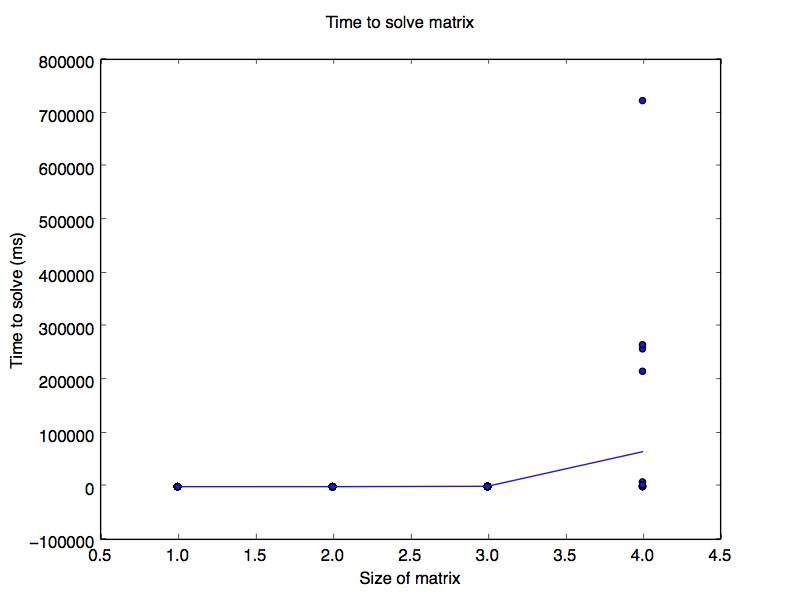
\includegraphics[width=\linewidth]{src/allN.jpg}

We can see the horrible exponential nature of this algorithm. The first 2 N have an almost 0 runtime. Taking it up to $N=3$ and $N=4$ we are able to see huge increases to the runtime. Its also important to note that this data through out all data that took too long to run. Doing a full search of the graph for a $N=3$ space can take an unfeasible amount of time. Even with this data being timed out we are still able to see the exponential nature of this NP-Complete algorithm.

\subsubsection{Application}
The proof above, for showing a runtime of $O(n^{2*n^4 + 2})$ is fairly straight forward but a runtime that is that exponential is horrible. To put in in perspective if it took 1 ms to calculate a sudoku for n = 1 then it would take 4 minutes to calculate a sudoku for n = 2, $2*10^70$ days to calculate a standard sudoku. Even though it does take a very long time for standard Sudoku it doesn't quite take this long. Lets investigate into the possible reasons for this discrepancy. 

The leading factor into such a strict runtime was the massive search space. However, above, we assumed that every box had a branching factor of $n^2$ for each block. This however is not exactly true. The first block does have a branching factor of $n^2$ but by selecting this value it decreases the branching factor for all sub trees that share a row, column or sub square with this block. 

What does this mean? Well essentially once we commit to a value in a given square it dramatically decreases the sub-trees that we need to search through. This was the point of the reject subroutine if you remember. To prune the tree of sub-trees we don't need to search because they can't have a solution. 

An example of this branching factor can be seen for the $n=2$ case below. 

\begin{center}
  \begin{tabular}{ | c | c | c | c | }
    \hline
    	4 & 3 & 2 & 1 \\ \hline
    	2 & 1 & 2 & 1 \\ \hline
    	2 & 2 & 1 & 1 \\ \hline
       	1 & 1 & 1 & 1 \\
    \hline
  \end{tabular}
\end{center}

Only one level actually has a $n^2$ branching factor the rest have a dramatic decrease. 

The same type of square can be shown for the $n = 3$ situation. 

\begin{center}
  \begin{tabular}{ | c | c | c | c | c | c | c | c | c |}
    \hline
    	9 & 8 & 7 & 6 & 5 & 4 & 3 & 2 & 1 \\ \hline
        7 & 6 & 5 & 6 & 5 & 4 & 3 & 2 & 1 \\ \hline
        3 & 2 & 1 & 3 & 2 & 1 & 3 & 2 & 1 \\ \hline
        6 & 5 & 4 & 6 & 5 & 4 & 3 & 2 & 1 \\ \hline
        5 & 4 & 3 & 6 & 5 & 4 & 3 & 2 & 1 \\ \hline
        3 & 2 & 1 & 3 & 2 & 1 & 3 & 2 & 1 \\ \hline
        3 & 2 & 1 & 3 & 2 & 1 & 3 & 2 & 1 \\ \hline
        2 & 2 & 1 & 2 & 2 & 1 & 2 & 2 & 1 \\ \hline
        1 & 1 & 1 & 1 & 1 & 1 & 1 & 1 & 1 \\ 
    \hline
  \end{tabular}
\end{center}

As we can see the branching factor is way better than the worst case proved in the proof above but it can not be generalized because the branching factor also depends on how many hints were given. This then forces us to analyze how we look at the runtime. 

\section{Runtime including Hints}
In order to improve on our $O(n^{2*n^4 + 2})$ runtime we need to start looking at Sudoku that are not empty matrices. To do this we can introduce a new variable m where m is the number of values that still need to be found. In the worst case we are given an empty board then $ m  n^4$. We can then turn the runtime into $n^{2m}$. 

For every hint that we are given then it dramatically shrinks the number of states by an order of magnitude. How exactly does this look then. Well we can look at two different types of Sudokus reasonably well.
The first chart shows how long it takes to run a sudoku assuming a n = 2. We can run the same kind of test as we ran above where we give the solver different numbers of hints and we see how long it takes to solve. 

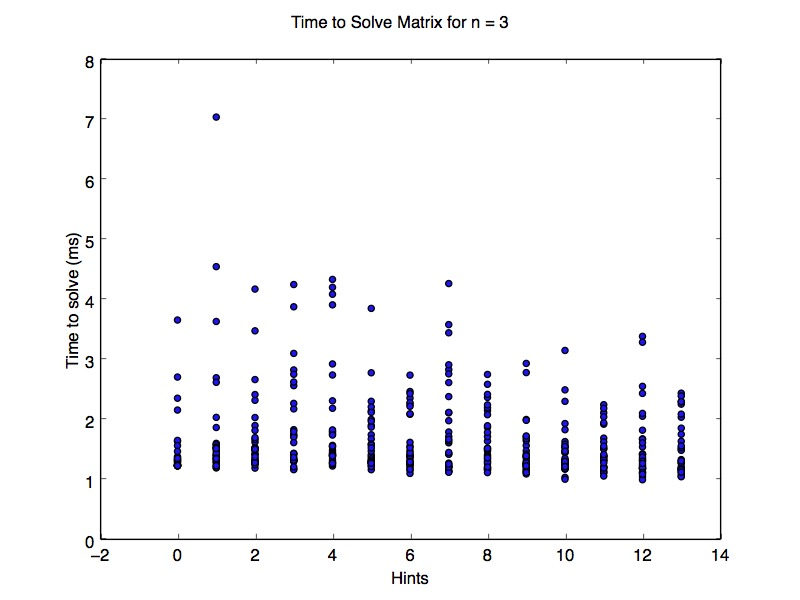
\includegraphics[width=\linewidth]{src/four.jpg}

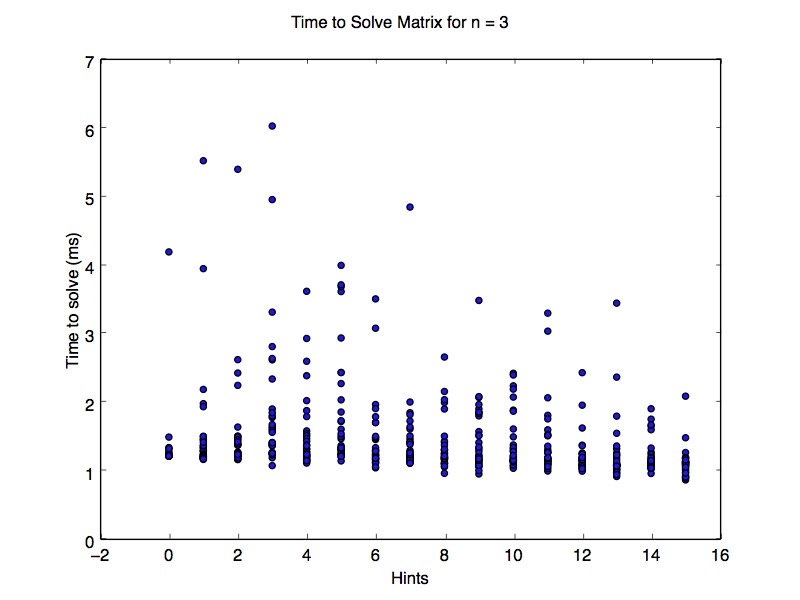
\includegraphics[width=\linewidth]{src/nine.jpg}

From these graphs we are able to see that the runtime greatly differs depending on the number of hints provided. However we should see the runtime dramatically decrease with the number of hints provided. We do see this behavior if we only look at the outliers for the $N=3$ graph but overall we see that the more hints that we provide the longer it takes for the backtracking algorithm to solve. This is a paradox because it contradicts what the math has shown. This discrepancy has a very simple explanation though. The worst case solution assumes that the algorithm will have to search the whole search space. In most cases though there are many solutions to a sudoku with few hints and there is a great chance that the algorithm will find one early through the searching process. I will not discuss this phenomenon in this paper but it is good to note that the search space rarely needs to be fully searched. 

\section{Space Complexity for size N}
The space complexity of the backtracking algorithm is extremely straight forward and nowhere near as complicated to analyze as the runtime. The space complexity depends on far less than the runtime and does not depend on the search space. To prove this we can analyze the algorithm by looking at it piece by piece. 

\subsubsection{Reject and Accept}
Reject like we have discussed before loops through all the elements 3 times. Each set of four loops creates a set for the elements to be added too. At any given time there is only one set, so we only need to worry about the potential elements added to each set. For a matrix of size n there are $n^2$ possible values. At the worst case we need to add all of these values to the set. Thus proving reject needs $O(n^2)$ space. 

\subsubsection{isEmpty and getIndices}
Both of these methods as I have mentioned have a constant math conversion and thus take up no space. 

\subsubsection{Sudoku Backtracking Algorithm}
The sudoku Backtracking algorithms space requirements can be defined by looking at when and where it creates memory. Looking at the algorithm 

\begin{algorithm}
\caption{Sudoku Backtracking}\label{solve}
\begin{algorithmic}[1]
\Procedure{solve}{G, box}

\If{reject (G)} -> Uses $n^2$ but removed after
\State return None
\EndIf

\If{accept(G)} -> Uses $n^2$ but removed after
\State return G
\EndIf

\If $box \ge n^4$  -> O(1)
\State return None
\EndIf

\State x, y = getIndices(box, size) -> O(1)

\If{ !self.isempty(G[x][y])}  -> O(1)
\State return solve(G, box+1) 
\EndIf

\For{ index $i < n^2$} -> O(1)
\State $G'$[x][y] = i
\State solution = solve($G'$, box + 1)
\If{result !=None}
\State return Result
\EndIf
\EndFor
\State G[x][y] = 0
\State Return None
\EndProcedure
\end{algorithmic}
\end{algorithm}

At each step in the graph search we can see that we need $O(n^2)$ space for the accept and reject subroutines. This is not carried down from recursive calls though and thus does not add over time. No space is actually needed to be saved into the recursive calls because all the sudoku backtracking is done in place. Thus we need $O(n^2) + O(n^4)$ showing that the space complexity for the sudoku backtracking algorithm is at most $O(n^4)$

We can take this a step further though to establish that not only is the space $O(n^4)$ but is also $\Theta(n^4)$ We can see that size of space is bounded both upper and lower by the size of $n^4$ we will never do any better that $n^4$ because that is the bare minimum that is required to hold all the information. We also wont do any worse as we showed above thus proving the $\Theta(n^4)$ space complexity. 

\subsection{Space Complexity for Different Hints}
Its also important to mention that the space complexity, unlike the runtime, does not change depending on the number of hints. Every step of the algorithm regardless of whether it is a hint or not starts with the recursive call. The algorithm loops through the reject and accept subroutines. All hints are contained inside the game matrix and thus the space Complexity is $\Theta(n^4)$ regardless the number of hints the player is given. 

%---------------------------------------------------
\subsection{Inputs} 

I mentioned briefly that the Algorithm for solving sudoku can very greatly depending on how much of the search tree it needs to search. If it only needs to search a small subset of the tree then the algorithm can perform extremely well. If it needs to search the whole space then the algorithm could take hours to solve a standard $n=3$. In order to explain this phenomena we can look at three types of inputs: Worst Case, Average Case, Best Case 


\subsubsection{Worst Case Input}
The absolute worst case input you could have is the input that does not have a solution but still requires a full tree search to determine that there is no solution. Of course most people would consider this to be cheating because the definition of Sudoku requires there to be a solution so we are only going to talk about worst case inputs. Of course our algorithm doesn't need this requirement but for the purposes of this next section we will assume there is a solution. 

Like we just talked about the worst case solution is to not have a solution and to discover this by searching the whole tree. Now because the definition of sudoku we need to look at the situation where there is definitely a solution. The worst case would be when you need to search the whole tree, aka no pruning, and the solution appears on the farther most right side. However, this situation is near impossible to generate because we cant remove pruning just for the analysis. So we can redefine the worst case input as an input which forces the algorithm to do the farthest depth search for each tree and that has a max value in each square as long as the matrix still follows the rules of sudoku. 

Why is this the case? Well an input that forces a deep search thus has to do lots of backtracks leading to an exponentially larger search space. By requiring each value be a max it means that the worst case input would have backtracked over all the lower value sub trees meaning that it has to keep searching through many trees. The algorithm searches low to high. 

	Mathematically we can then define the worst input graph G, solve(G) where solving G maximizes number of backtracks. 
    
    We can see that here with this example. This example is the worst case generated for the $n=2$ example. This was the longest $n=2$ puzzle and it took 6.69 ms to solve.
    
\begin{center}
  \begin{tabular}{ | c | c | c | c | }
    \hline
		& & & \\ \hline
        1 & & &  \\ \hline
        & & & \\ \hline
        3 & & & 1 \\
    \hline
  \end{tabular}
\end{center}

The solution for this puzzle is: 

\begin{center}
  \begin{tabular}{ | c | c | c | c | }
    \hline
		2 & 3 & 1 & 4\\ \hline
        1 & 4 & 2 & 3 \\ \hline
        4 & 1 & 3 & 2\\ \hline
        3 & 2 & 4 & 1 \\
    \hline
  \end{tabular}
\end{center}

We can see by looking at the first recursion level. That at almost every box there was the max number of recursion possible given the number of hints. This forces the puzzle to take a long time to solve. 

Just in comparison this next example is the longest $n=3$ puzzle that we were able to solve. It took over 1.5 hours to solve. There are longer puzzles in existence but were not able to solve them due to time constraint. 

\begin{center}
  \begin{tabular}{ | c | c | c | c | c | c | c | c | c |}
    \hline
    	 &  & 5 &  &  &  &  &  &  \\ \hline
        6 &  &  &  &  &  &  &  &  \\ \hline
        &  &  &  &  &  &  &  &  \\ \hline
   		 &  &  &  &  &  &  &  &  \\ \hline
         & 6 &  & 1 &  &  &  &  &  \\ \hline
        7 &  &  &  &  &  &  &  &  \\ \hline
      	 & 5 &  &  & &  &  &  & 8 \\ \hline
         &  & 6 & &  &  &  & 1 &  \\ \hline
        9 &  &  & 3 & 1 &  &  &  & 7 \\ 
    \hline
  \end{tabular}
\end{center}

\subsubsection{Best Case Input}

Contrasting the worst case situation 
The best case puzzle is any puzzle that is fully filled in. Now obviously a fully filled in puzzle would be the best case situation but that doesn't help with any analysis. So just like the worst case example we need to broaden the definition. Mathematically we can define the best case input to be any puzzle that the algorithm never searches a sub tree where a solution does not exist. 

What does this mean in normal terms. Well essentially what we can learn from the best case definition is that the fastest puzzle is a puzzle where the algorithm "Guesses" each squares value on the first attempt. There will be no backtracking for this "Best Case Input". 

Lets walk through the best case $n=2$ example. This puzzle took 0.8 ms to solve. 

\begin{center}
  \begin{tabular}{ | c | c | c | c | }
    \hline
		2 & 4 &  & \\ \hline
         &  &  &  \\ \hline
         &  &  & 2\\ \hline
        4 & 2 & 1 & 3 \\
    \hline
  \end{tabular}
\end{center}

Looking at this puzzle we can see that every single square has only one possible value leading the algorithm to guess its value on the first iteration. 

The best $n=3$ puzzle that was found was the following. It took 32 ms to solve this puzzle. 

\begin{center}
  \begin{tabular}{ | c | c | c | c | c | c | c | c | c |}
    \hline
    	 & 7 &  &  &  &  & 8 &  &  \\ \hline
         &  &  &  &  &  &  & 6 &  \\ \hline
         &  &  & 4 &  &  &  &  &  \\ \hline
   		 &  &  &  &  &  & 7 &  &  \\ \hline
         &  &  &  &  &  &  &  &  \\ \hline
         & 1 & &  &  &  & 4 &  &  \\ \hline
      	 &  &  &  &  &  &  & 7 &  \\ \hline
         &  &  &  &  &  &  &  &  \\ \hline
         &  &  &  &  &  &  &  &  \\ 
    \hline
  \end{tabular}
\end{center}

\subsubsection{Inputs Average Case}
Now that we have a worst case and best case defined we can talk about the average case. While solving Sudoku we rarely see cases as black and white as the best and worst case. Most Sudoku don't have a lot of options per square because there is only one solution in typical sudoku. We see from experimental values that most Sudoku are average case. Looking at the runtime chart for different sizes of Sudoku. 

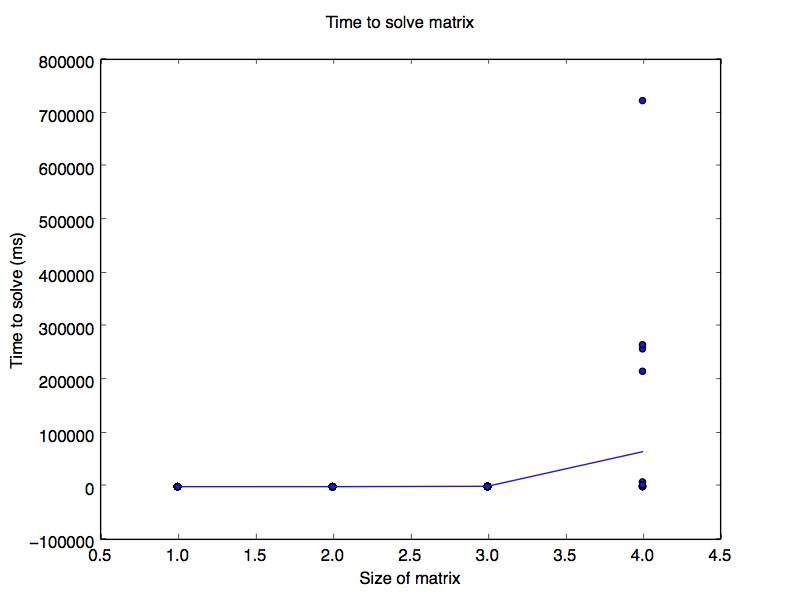
\includegraphics[width=\linewidth]{src/allN.jpg}

We can see that even though some Sudoku have extra long solve times. The majority get solved extremely quickly. The average sudoku takes 127 ms to solve. 

Why is this? Like I mentioned above there are only one solution for the average case sudoku. In order to ensure that there is only one solution there needs to be a sufficient amount of hints to ensure this constraint. Adding these hints prevent the algorithm from having to search the full search tree. Instead it is able to very efficiently find the correct solution. 

Using this information we are able to mathematically define the average case sudoku as any sudoku that has only one valid solution. 

\section{Recent Work}
Backtracking algorithms can be applied to a variety of problems and as we have learned can be used to solve sudoku but it is not always the best thing to do. In recent years there has been work into highly specialized algorithms to solve sudoku. One of these algorithms is knows as Crooks Algorithm.

Crooks algorithm, at a high level, works the exact same way humans are used to solving Sudoku. It goes through each square and using the hints determines the possible values that each square can have. Then it performs a coloring algorithm but instead of always starting at the first box. It starts at the values that have the fewest possible options. 
\cite{Crook2}

\section{Conclusions}
In conclusion I have a successfully created a Sudoku backtracking implementation. The implementation and given pseudocode has a worst case runtime of $O(n^{2*^{n^4} + 2})$. This runtime is shown because the search space of a Sudoku puzzle is $O(n^2*^{n^4} + 2)$. $n^2$ because each tree level has $n^2$ possible branches and raised to the $n^4$ because this is the tree depth. Admitting that this runtime is extremely bad we were able to improve on it by introducing a variable m where m is the number of empty boxes we are able to lower the runtime to $O(n^2*m)$. This is still exponential but unfortunately by the nature of the backtracking algorithm we can not do any better. 

In addition to proving this runtime I successfully proved a space complexity of $O(n^4)$ for the given algorithm. This complexity comes from the fact that the algorithm uses in place calculations and thus never grows its need for space. The algorithm keeps track of a $n^4$ sized matrix and at each level uses a $O(n^2)$ sized set to ensure all the rules are met.  

Finally we were able to analyze the best, average, and worst case inputs and how often they occur. We determined that worst case input is a puzzle that forces the algorithm to have the most backtracked trees. The average case makes up most of the puzzles and allows for one solution that the hints easily map out. Lastly, the best case input is one where the backtracking algorithm correctly guesses the boxes value on the first try preventing the algorithm from having to backtrack sub trees. 

%\end{document}  % This is where a 'short' article might terminate


%
% The following two commands are all you need in the
% initial runs of your .tex file to
% produce the bibliography for the citations in your paper.
\cite{*}
\bibliographystyle{abbrv}
\bibliography{sigproc}  % sigproc.bib is the name of the Bibliography in this case
% You must have a proper ".bib" file
%  and remember to run:
% latex bibtex latex latex
% to resolve all references
%
% ACM needs 'a single self-contained file'!
%
%APPENDICES are optional
%\balancecolumns
\end{document}
